\documentclass{standalone}
\usepackage[T1]{fontenc}
\usepackage[utf8]{inputenc}
\usepackage{pgf,tikz}
\usepackage{setspace}
\usepackage{pgfplots}
\usepgfplotslibrary{groupplots}

\pgfplotsset{compat=1.13}

\makeatletter
\newcommand*{\rom}[1]{\expandafter\@slowromancap\romannumeral #1@}
\makeatother

\begin{document}
   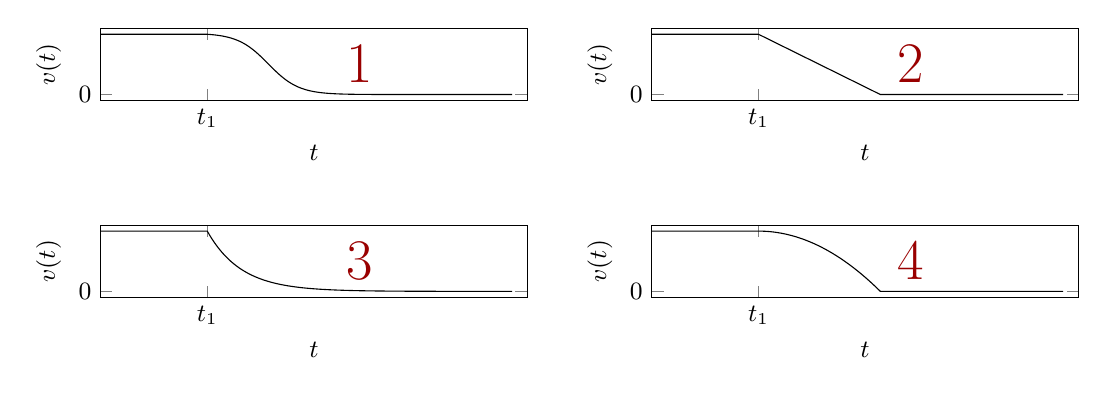
\begin{tikzpicture}
   \small

   \begin{axis}[
   width=7cm,
   height=2.5cm,
   xlabel={$t$},
   ylabel={$v(t)$},
   xmin=-3.5,
   xmax=10.5,
   ytick = {0},
   xtick = {0},
   xticklabels = {$t_1$},
   ]
   \addplot+[black, no marks, domain=-4:10, samples=400,variable=k] { (k < 0) + (k>0)*(1+exp(-4))/(1+exp(4*(0.5*k-1)))};

   \node[black!40!red] at (axis cs: 5, 0.5) {\huge 1};
   \end{axis}

   \begin{axis}[
   xshift=7cm,
   width=7cm,
   height=2.5cm,
   xlabel={$t$},
   ylabel={$v(t)$},
   xmin=-3.5,
   xmax=10.5,
   ytick = {0},
   xtick = {0},
   xticklabels = {$t_1$},
   ]
   \addplot+[black, no marks, domain=-4:10, samples=400,variable=k] { (k<0) + ((k>=0) - (k>4))*(1/4*(4-k)) };
   \node[black!40!red] at (axis cs: 5, 0.5) {\huge 2};
   \end{axis}

   \begin{axis}[
   xshift=0cm,
   yshift=-2.5cm,
   width=7cm,
   height=2.5cm,
   xlabel={$t$},
   ylabel={$v(t)$},
   xmin=-3.5,
   xmax=10.5,
   ytick = {0},
   xtick = {0},
   xticklabels = {$t_1$},
   ]
   \addplot+[black, no marks, domain=-4:10, samples=400,variable=k] { (k<0) + (k>0)*exp(-0.9*k)};
   \node[black!40!red] at (axis cs: 5, 0.5) {\huge 3};
   \end{axis}

   \begin{axis}[
   xshift=7cm,
   yshift=-2.5cm,
   width=7cm,
   height=2.5cm,
   xlabel={$t$},
   ylabel={$v(t)$},
   xmin=-3.5,
   xmax=10.5,
   ytick = {0},
   xtick = {0},
   xticklabels = {$t_1$},
   ]
   \addplot+[black, no marks, domain=-4:10, samples=400,variable=k] { (k<0) + ((k>=0) - (k>4))*(1-1/16*pow(-k,2)) };
   \node[black!40!red] at (axis cs: 5, 0.5) {\huge 4};
   \end{axis}


   \end{tikzpicture}

 \end{document}
 